\documentclass[../ro-fa-lab.tex]{subfiles}

% !TeX spellcheck = ro_RO
\usepackage{ucs}
\usepackage{amsmath}
\usepackage{amsfonts}
\usepackage{amssymb}
\usepackage{graphicx}

\usepackage{hyperref}
\hypersetup{
    pdftitle={(RO) L9 - BFS},   % The title shown in the browser tab
    pdfauthor={},         % Your name or organization
    pdfsubject={},   % A brief description
    pdfkeywords={}
}

\begin{document}


\section{\texorpdfstring{\textbf{Tema Nr. 9: Căutarea în lățime (BFS)}}{Tema Nr. 9: Căutarea în lățime (BFS)}}\label{assign9}


\subsection{Introducere}
În acest laborator se va implementa algoritmul BFS (căutarea în lățime), conform secțiunii 22.2 din Cormen.

\subsection{Structura proiectului}
La acest laborator veți porni de la 3 fișiere:
\begin{itemize}
    \item \texttt{main.cpp} - sursa principală, responsabilă cu interfața de vizualizare
    \item \texttt{bfs.h} - definiții pentru tipuri de structuri și funcții
    \item \texttt{bfs.cpp} - implementarea algoritmilor
    \item \texttt{grid.txt} - labirintul care va fi afișat și traversat
    \item \texttt{Profiler.h} - biblioteca pentru numărarea operațiilor și pentru grafice
\end{itemize}


\textbf{!!!} Pentru rezolvarea cerințelor trebuie să faceți modificări doar în \texttt{bfs.cpp}.

Pentru a vizualiza mai ușor funcționarea algoritmului, \texttt{main.cpp} va afișa o interfață de tip text, în care se va vedea o un labirint ce trebuie traversat (celulele negre sunt libere iar cele albe sunt pereți).

\subsubsection{Inițializarea proiectului pe Windows, cu Visual Studio}
\begin{figure}[h]
    \centering
    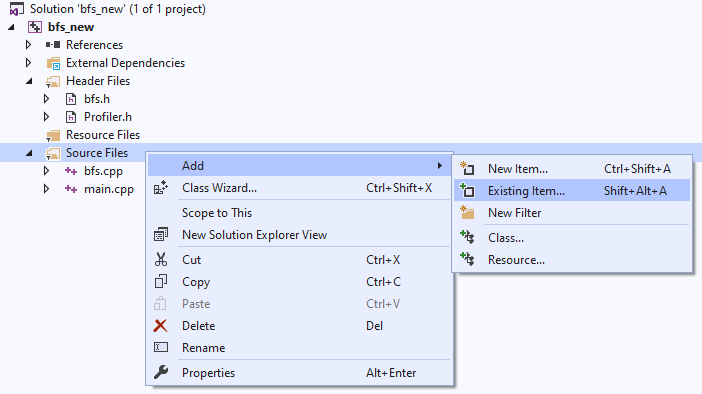
\includegraphics[width=9cm]{../Resources/lab9/vs_solution.png}
    \caption{Fereastra \textit{``Solution Explorer''} în Visual Studio}
    \label{fig:vs}
\end{figure}

Creați un proiect nou în Visual Studio, de tipul \textit{``Empty Project''} și copiați fișierele de mai sus în folderul proiectului.

Adăugați cele doua fișiere \texttt{.h} la secțiunea \textit{``Header Files''} și cele două fișiere \texttt{.cpp} la secțiunea \textit{``Source Files''}, efectuând click dreapta $\rightarrow$ \textit{``Add''} $\rightarrow$ \textit{``Existing Item''}, ca în Figura~\ref{fig:vs}.

\subsubsection{Inițializarea proiectului pe Linux și Mac}
Puteți edita fișierele proiectului cu orice editor doriți. Proiectul conține și un fișier \texttt{Makefile}, deci este suficient să rulați comanda \texttt{make} pentru compilarea acestuia. Executabilul \texttt{.exe} rezultat se va numi \texttt{main}, și se poate rula în terminal, executând \texttt{./main}.

\subsection{Funcționare}
La pornirea programului se va afișa labirintul, în mod similar cu Figura~\ref{fig:grid1}.

\begin{figure}[h]
    \centering
    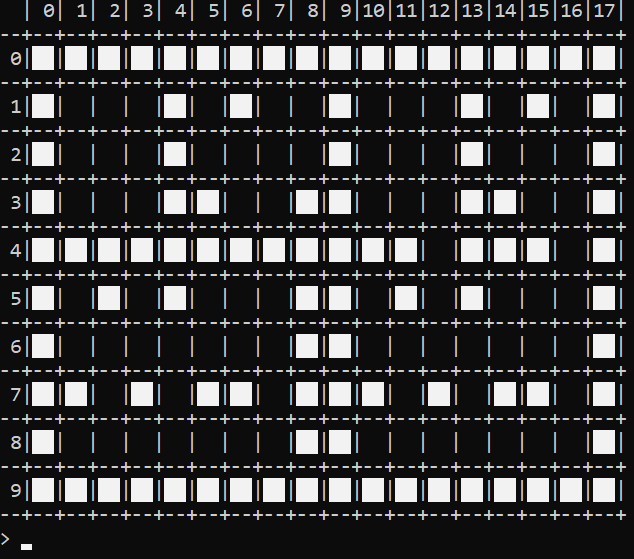
\includegraphics[width=7cm]{../Resources/lab9/grid1.png}
    \caption{Interfața programului}
    \label{fig:grid1}
\end{figure}

În partea de jos, utilizatorul poate tasta una din comenzile de mai jos:
\begin{itemize}
    \item \texttt{exit}\\
        terminarea programului
    \item \texttt{clear}\\
        curățarea informațiilor anterioare din grilă
    \item \texttt{neighb <row> <col>} \\
        se vor afișa vecinii celulei de pe linia \texttt{<row>} și coloana \texttt{<col>}.
    \item \texttt{bfs <row> <col>} \\
        se va efectua o parcurgere BFS, pornind de la celula de la linia \texttt{<row>} și coloana \texttt{<col>}.
    \item \texttt{bfs\_step <row> <col>} \\
        la fel ca la \texttt{bfs}, dar rezultatul se va afișa pas cu pas, în funcție de distanța față de sursă
    \item \texttt{bfs\_tree <row> <col>} \\
        la fel ca la \texttt{bfs}, dar se va afișa și arborele BFS sub grilă
    \item \texttt{path <row1> <col1> <row2> <col2>} \\
        se va afișa cel mai scurt drum între celulele \texttt{(<row1> <col1>)} și \texttt{(<row2> <col2>)}
    \item \texttt{perf} \\
        se vor genera graficele pentru evaluarea performanței algoritmului
\end{itemize}

\subsubsection{Exemplu: comanda \texttt{neighb}}
Dacă se rulează:\\
\texttt{neighb 2 3}
ar trebui să apară imaginea din Figura~\ref{fig:neighb}.

\begin{figure}[h]
    \centering
    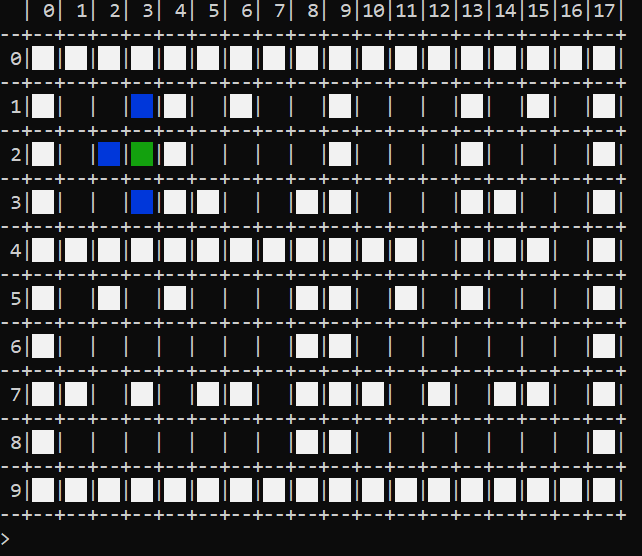
\includegraphics[width=7cm]{../Resources/lab9/grid_neighb.png}
    \caption{Rezultatul comenzii \texttt{neighb 2 3}}
    \label{fig:neighb}
\end{figure}

Celula de start se va colora cu verde, iar vecinii acesteia cu albastru.

În momentul de față funcția \texttt{get\_neighbors()} nu este implementată, deci nu se va afișa rezultatul dorit. Puteți verifica dacă ați implementat corect această funcție rulând comanda pentru diverse celule. Fiecare celulă va avea maxim 4 vecini (sus, jos, stânga, dreapta), și nu trebuie afișate celule din afara grid-ului sau celule care conțin pereți.

\subsubsection{Exemplu: comenzile \texttt{bfs} și \texttt{bfs\_step}}
Dacă se rulează:\\
\texttt{bfs 6 3}
ar trebui să apară imaginea din Figura~\ref{fig:bfs1}.

\begin{figure}[h]
    \centering
    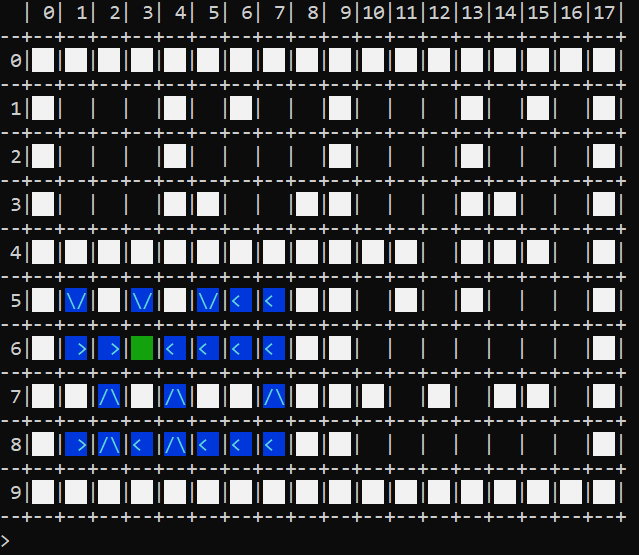
\includegraphics[width=7cm]{../Resources/lab9/grid_bfs1.png}
    \caption{Rezultatul comenzii \texttt{bfs 6 3}}
    \label{fig:bfs1}
\end{figure}

Celula de start se va colora cu verde, iar celulele parcurse se vor colora cu albastru. Pe fiecare celulă albastră va apărea o săgeată care va indica în ce direcție se află părintele din arborele BFS.

În momentul de față funcția \texttt{bfs()} nu este implementată, deci nu se va afișa rezultatul dorit. Puteți verifica dacă ați implementat corect această funcție rulând comanda pentru diverse celule.

\subsubsection{Exemplu: comanda \texttt{bfs\_tree}}
Dacă se rulează:\\
\texttt{bfs 2 6}
ar trebui să apară imaginea din Figura~\ref{fig:bfs_tree}.

\begin{figure}[h]
    \centering
    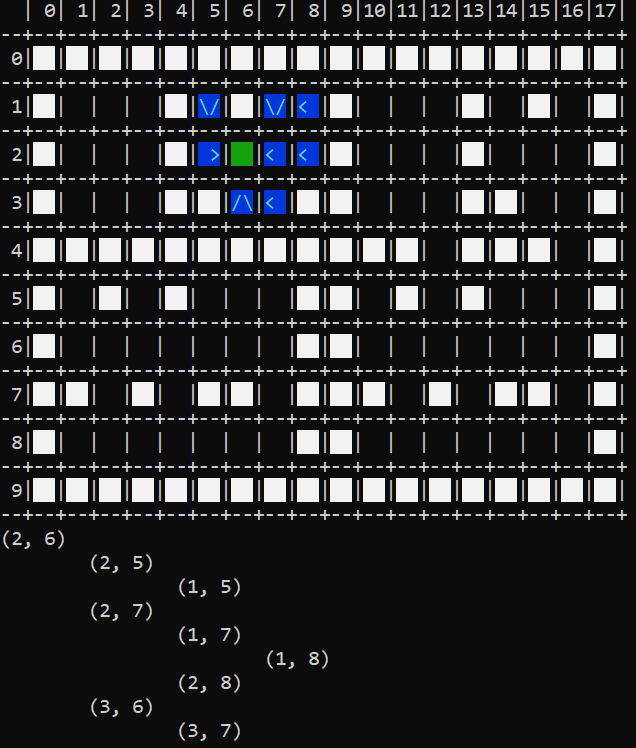
\includegraphics[width=7cm]{../Resources/lab9/grid_bfs_tree.png}
    \caption{Rezultatul comenzii \texttt{bfs\_tree 2 6}}
    \label{fig:bfs_tree}
\end{figure}

Rădăcina arborelui este nodul de start, respectiv \texttt{(2, 6)}. Copii acestui nod, sunt nodurile în care se poate ajunge direct din rădăcină: \texttt{(2, 5)}, \texttt{(2, 7)} și \texttt{(3, 6)} (ordinea acestora poate să difere în altă implementare).

\subsubsection{Exemplu: comanda \texttt{path}}
Dacă se rulează:\\
\texttt{path 5 10 3 15}
ar trebui să apară imaginea din Figura~\ref{fig:path}.

\begin{figure}[h]
    \centering
    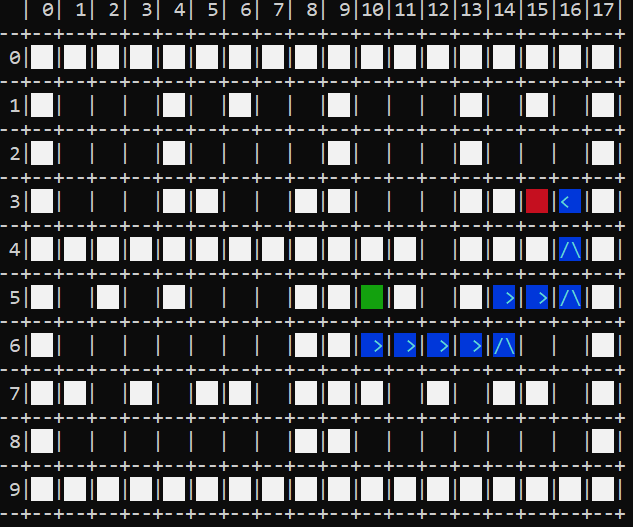
\includegraphics[width=7cm]{../Resources/lab9/grid_path.png}
    \caption{Rezultatul comenzii \texttt{path 5 10 3 15}}
    \label{fig:path}
\end{figure}

Celula de start se va colora cu verde, cea de final cu roșu, iar celulele care fac parte din drumul cel mai scurt se vor colora cu albastru. Pe fiecare celulă albastră va apărea o săgeată care va indica direcția de mers.

În momentul de față funcțiile \texttt{shortest\_path()} și \texttt{bfs()} nu sunt implementate, deci nu se va afișa rezultatul dorit. Puteți verifica dacă ați implementat corect aceste funcții rulând comanda pentru diverse perechi de celule.

\subsubsection{Structuri de date folosite}
În fișierul \texttt{bfs.h} sunt definite câteva structuri de date utile în cadrul framework-ului.

Structura \texttt{Grid} modelează o grilă, formată din \texttt{rows} linii și \texttt{cols} coloane, elementele acesteia fiind în matricea \texttt{mat}. O celulă liberă va avea valoarea 0, iar una ce conține un perete va avea valoarea 1.

Structura \texttt{Point} modelează un punct sau o celulă din grilă, câmpurile \texttt{row} și \texttt{col} reprezentând linia și coloana la care se află.

Structura \texttt{Node} modelează un nod din graf și conține următoarele câmpuri:
\begin{itemize}
    \item \texttt{position} de tip \texttt{Point} reprezintă celula din grilă corespunzătoare nodului.
    \item \texttt{adjSize} - numărul de vecini ai nodului respectiv
    \item \texttt{adj} - vectorul de vecini, de dimensiune \texttt{adjSize}
    \item \texttt{color} - culoarea nodului; la început toate nodurile au culoarea \texttt{COLOR\_WHITE}, adică valoarea 0
    \item \texttt{dist} - distanța față de nodul de start, în parcurgerea BFS
    \item \texttt{parent} - pointer la nodul părinte, în arborele BFS
\end{itemize}

Structura \texttt{Graph} modelează un graf și conține numărul de noduri \texttt{nrNodes} și vectorul \texttt{v} cu pointeri spre acestea.

\subsection{Cerințe}

\subsubsection{Determinarea vecinilor unei celule (2p)}

În \texttt{bfs.cpp}, trebuie completată funcția \texttt{get\_neighbors()} care primește ca parametri un pointer la structura de tip \texttt{Grid}, un punct \texttt{p} de tip \texttt{Point} și un vector de puncte \texttt{neighb} care se va completa cu vecinii punctului \texttt{p}. Funcția va returna numărul de vecini completați în vectorul \texttt{neighb}.

Un punct din grilă va avea maxim 4 vecini (sus, jos, stânga, dreapta). Nu toți vecinii sunt valizi: unii vecini pot ajunge în afara grilei (coordonate negative, sau peste dimensiuni) sau pot fi în interiorul unui zid. Din acest motiv, după ce calculați poziția unui vecin, ar trebui să verificați că aceasta cade în interiorul grilei, apoi că aceasta este liberă (valoarea din matrice la poziția respectivă e 0).

Vecinii valizi se vor completa în vectorul \texttt{neighb}. Se garantează că la apelul funcției din framework, acesta va avea cel puțin 4 elemente, deci nu se poate depăși capacitatea acestuia. Deoarece numărul de vecini completați poate fi mai mic de 4, trebuie să returnăm numărul acestora.

\subsubsection{Implementarea algoritmului BFS (3p)}
În \texttt{bfs.cpp}, trebuie completată funcția \texttt{bfs()} care primește ca parametri un pointer la structura de tip \texttt{Graph} și nodul de start \texttt{s} de tip \texttt{Node*}. Funcția va aplica algoritmul BFS conform secțiunii 22.2 din Cormen.

Nodurile din graf au la început culoarea \texttt{COLOR\_WHITE}, iar câmpurile \texttt{dist} și \texttt{parent} sunt inițializate cu 0, respectiv \texttt{NULL}. După parcurgere, toate nodurile la care se poate ajunge din nodul de start trebuie să aibă culoarea \texttt{COLOR\_BLACK}, distanța \texttt{dist} setată pe numărul de pași de la nodul de start până la nodul respectiv, iar pointerul \texttt{parent} trebuie să indice părintele în arborele BFS.

\subsubsection{Afișarea arborelui BFS (2p)}
În \texttt{bfs.cpp}, trebuie completată funcția \texttt{print\_bfs\_tree()} care primește ca parametru un pointer la structura de tip \texttt{Graph} pe care s-a rulat deja algoritmul BFS, deci culorile nodurilor și părinții sunt deja setate.

În funcția data, este deja implementată construcția unui vector de părinți \texttt{p}, în care nodurile colorate cu negru în parcurgerea BFS vor fi numerotate de la $0$ la $n$. Deasemenea se construiește vectorul \texttt{repr} care conține coordonatele fiecărui nod. 

Pentru afișarea acestui arbore se poate adapta codul din laboratorul de arbori multi-căi.

\subsubsection{Evaluarea performanței algoritmului BFS (3p)}
Funcția \texttt{performance()} realizează numărarea operațiilor, variind pe rând numărul de muchii, respectiv numărul de vârfuri al grafului. Pentru fiecare valoare, trebuie să implementați construcția unui graf aleator, conex, care să aibă numărul respectiv de vârfuri și de muchii.

În interiorul funcției \texttt{bfs()} va trebui să implementați numărarea propriu-zisă a operațiilor, folosind parametrul opțional \texttt{op}. Deoarece acest parametru este opțional, uneori funcția \texttt{bfs()} va fi apelată din framework cu valoarea acestuia setată pe \texttt{NULL}. Din acest motiv, atunci când numărați o operație, verificați tot timpul că \texttt{op} e un pointer valid, ca în exemplul de mai jos:
\begin{verbatim}
    if(op != NULL) op->count();
\end{verbatim}

\subsubsection{Bonus: Determinarea celui mai scurt drum (0.5p)}
În \texttt{bfs.cpp}, trebuie completată funcția \texttt{shortest\_path()} care primește ca parametri un pointer la structura de tip \texttt{Graph}, nodurile de început și sfârșit \texttt{start} și \texttt{end} de tip \texttt{Node*}, respectiv vectorul \texttt{path}, ca parametru de ieșire în care se vor completa nodurile de pe traseu, în ordine. Funcția va returna numărul de noduri completate în vectorul \texttt{path}.

Pentru determinarea celui mai scurt drum între două noduri, se recomandă folosirea algoritmului BFS, implementat anterior, apoi reconstrucția drumului mergând din părinte în părinte în arborele BFS.

Vectorul \texttt{path}, în care se completează traseul, va avea o lungime de minim 1000 de elemente, la apelarea funcției. Returnați numărul de elemente care au fost completate în el, sau $-1$ în cazul în care nu se poate ajunge la nodul \texttt{end} pornind de la nodul \texttt{start}.

\subsubsection{Bonus: Unde poate ajunge un cal pe tablă? (0.5p)}
Folosind framework-ul dat, arătați că un cal poate ajunge pe orice poziție a unei table de șah goale, pornind din colțul din stânga-sus. Dați exemple de tablă care să conțină poziții libere la care nu se poate ajunge.

\end{document}